\newpage
\begin{tcolorbox}[enhanced,
  colback=blue!50!white, colframe=blue!25!black, coltext=white,
  fontupper=\Large\bfseries, arc=8mm, boxrule=0mm, boxsep=4mm]
  {\sffamily\LARGE Welcome} \label{Welcome}
\end{tcolorbox}


    \begin{minipage}{0.3\textwidth}
      \begin{center}
        \begin{tikzpicture}
          \begin{scope}
            \clip [rounded corners=2cm] (0,0) rectangle coordinate (centerpoint) (4cm,4cm); 
            \node [inner sep=0pt] at (centerpoint) {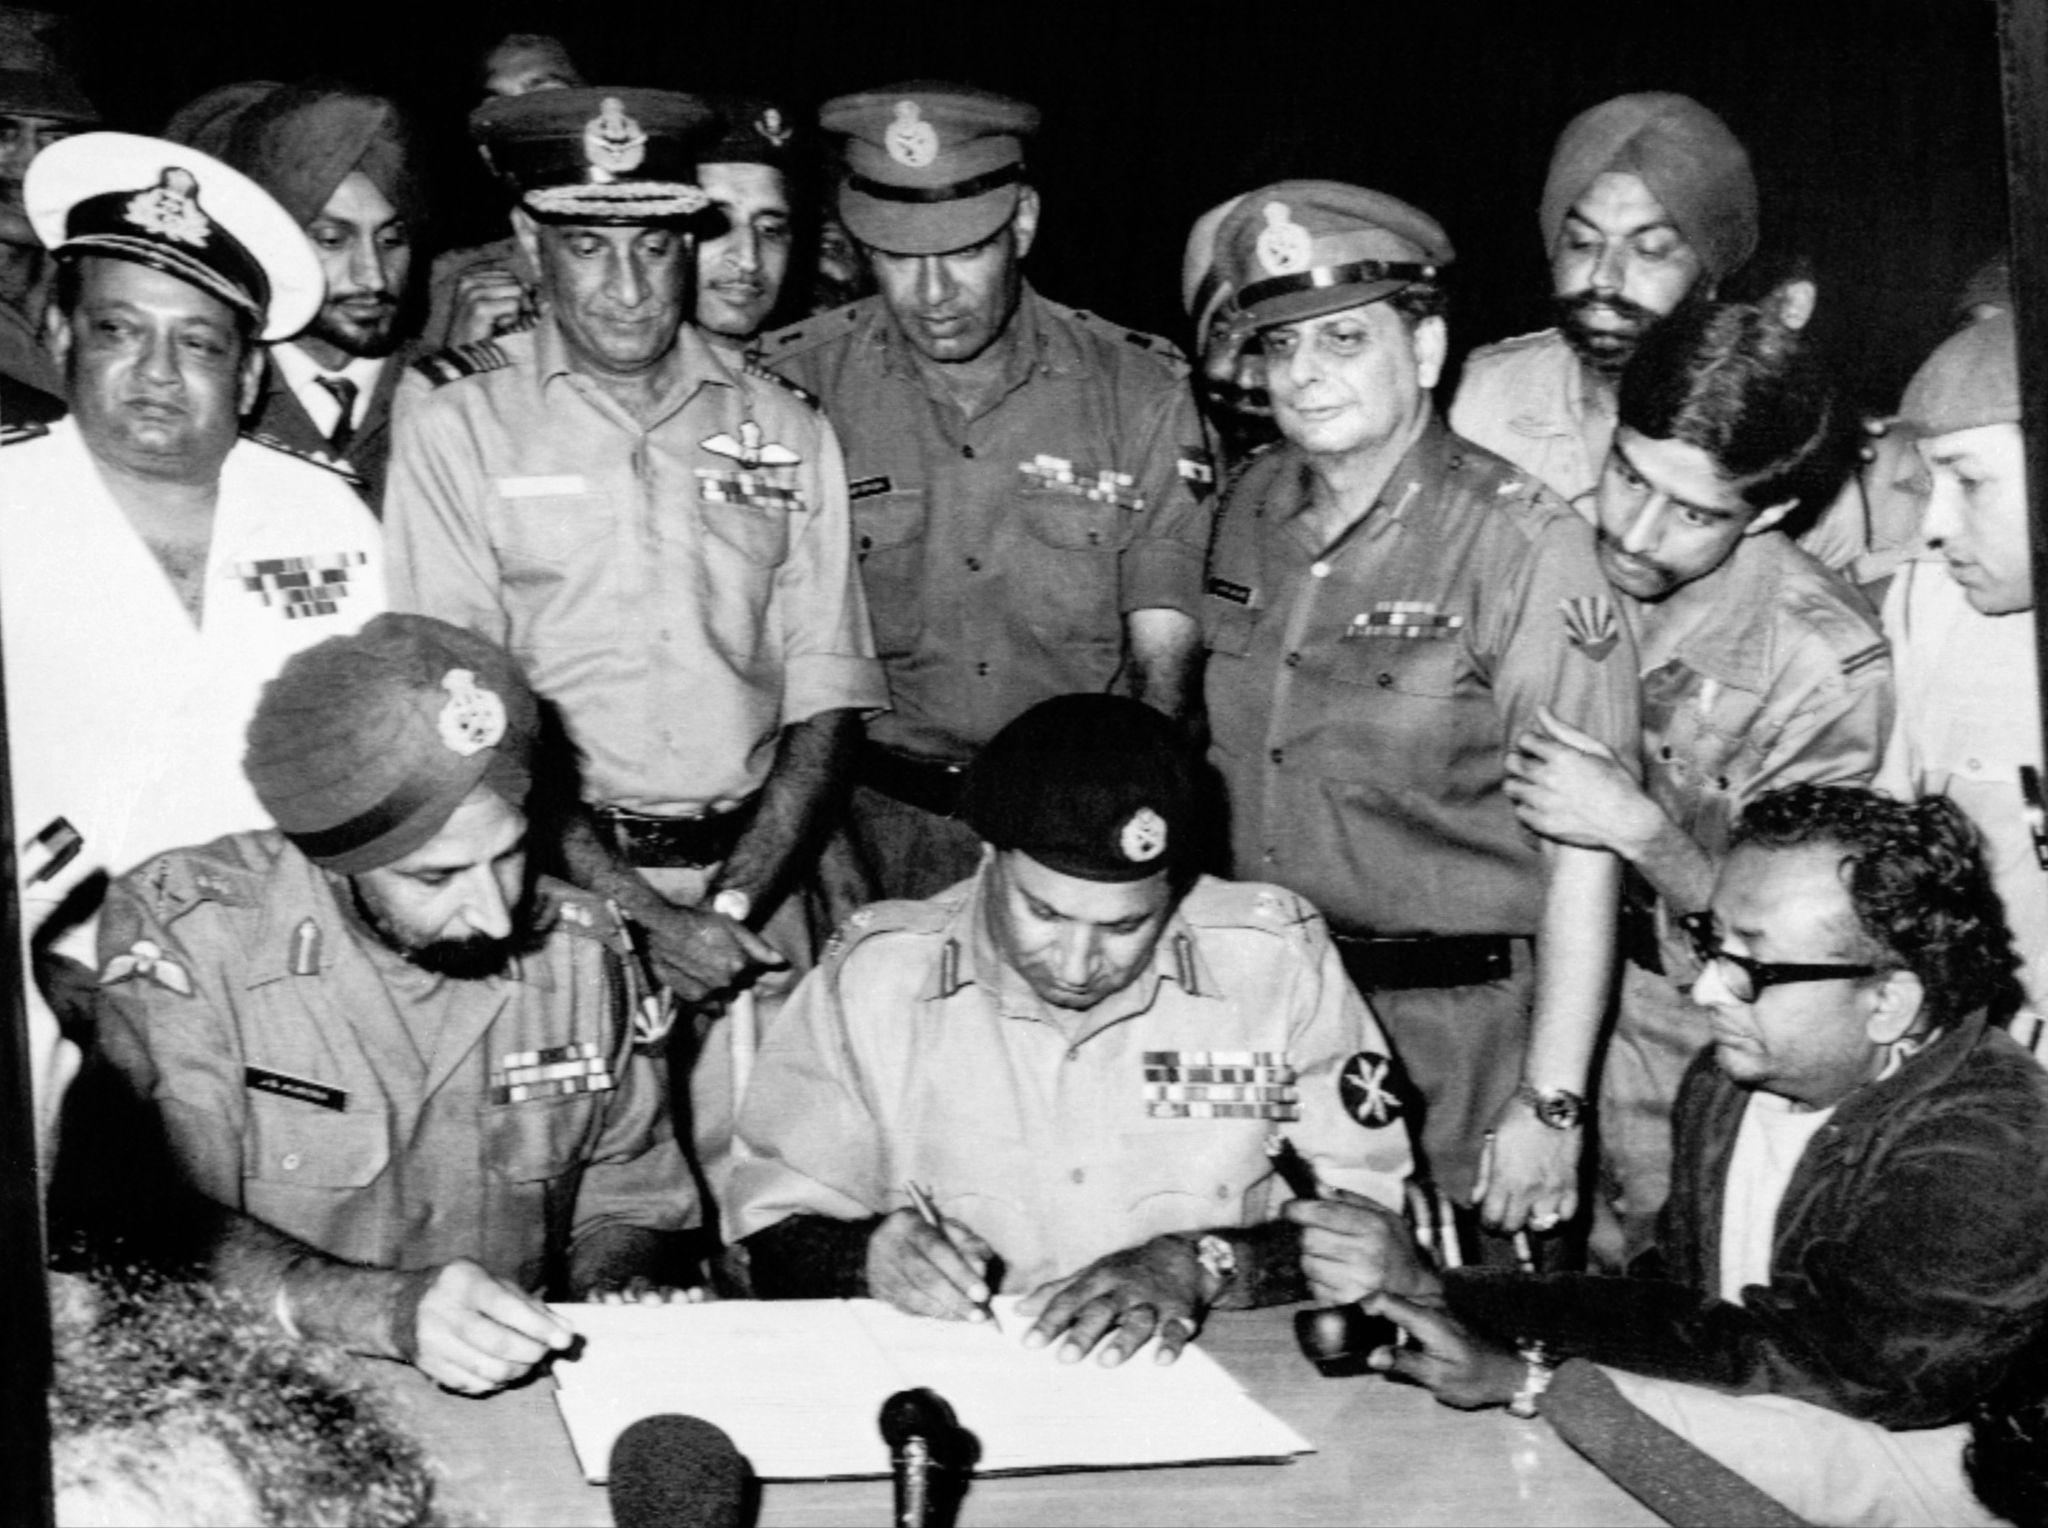
\includegraphics[width=4cm]{resources/head_of_department.jpeg}}; 
          \end{scope}
        \end{tikzpicture}
        \vspace{4cm}
      \end{center}
    \end{minipage}
    \hfill
\begin{minipage}{0.6\textwidth}
{\sffamily\justifying
\noindent

\vspace{1cm}

Dear all,\\

As we celebrate the spirit of India?s Independence on August 15, we are reminded that freedom is not merely political?it is also intellectual. Mathematics, in its purest form, liberates our thinking, allowing us to explore ideas beyond boundaries. Our nation?s progress rests on such intellectual independence, where curiosity and creativity light the path forward.\\

Coincidentally, the very next day marks the birth anniversary of Arthur Cayley, whose pioneering work in algebraic structures reshaped modern mathematics. His vision reminds us that transformative ideas often arise when we dare to imagine the unseen.\\

It is my privilege to release the second issue of our 2025 newsletter at this confluence of national pride and mathematical heritage. May we channel both the courage of our freedom fighters and the brilliance of our mathematical pioneers in every endeavour.\\

\noindent
 Best Wishes,\\
Dr. Jayesh M. Dhodiya}
\end{minipage}


\begin{minipage}{0.65\textwidth}
  Dear all,

As we celebrate the spirit of India?s Independence on August 15, we are reminded that freedom is not merely political?it is also intellectual. Mathematics, in its purest form, liberates our thinking, allowing us to explore ideas beyond boundaries. Our nation?s progress rests on such intellectual independence, where curiosity and creativity light the path forward.

Coincidentally, the very next day marks the birth anniversary of Arthur Cayley, whose pioneering work in algebraic structures reshaped modern mathematics. His vision reminds us that transformative ideas often arise when we dare to imagine the unseen.

It is my privilege to release the second issue of our 2025 newsletter at this confluence of national pride and mathematical heritage. May we channel both the courage of our freedom fighters and the brilliance of our mathematical pioneers in every endeavour.

Best Wishes

Dr. Jayesh M. Dhodiya
\end{minipage}

      \begin{minipage}{0.3\textwidth}
        \begin{center}
          \begin{tikzpicture}
            \begin{scope}
              \clip [rounded corners=2cm] (0,0) rectangle coordinate (centerpoint) (4cm,4cm); 
              \node [inner sep=0pt] at (centerpoint) {
\includegraphics[width=4cm]{resources/faculty_coordinator.png}}; 
            \end{scope}
          \end{tikzpicture}
          \vspace{4cm}
        \end{center}
      \end{minipage}
      \hfill

\vspace{1cm}
